\begin{figure}[h!]
    \centering
    \caption{Estimated shares pocketed by landlords under counterfactual MW policies, 
             Chicago-Naperville-Elgin CBSA}
    \label{fig:map_chicago_cf_shares}

    \begin{subfigure}{.5\textwidth}
        \caption{Increase in federal MW to \$9}
        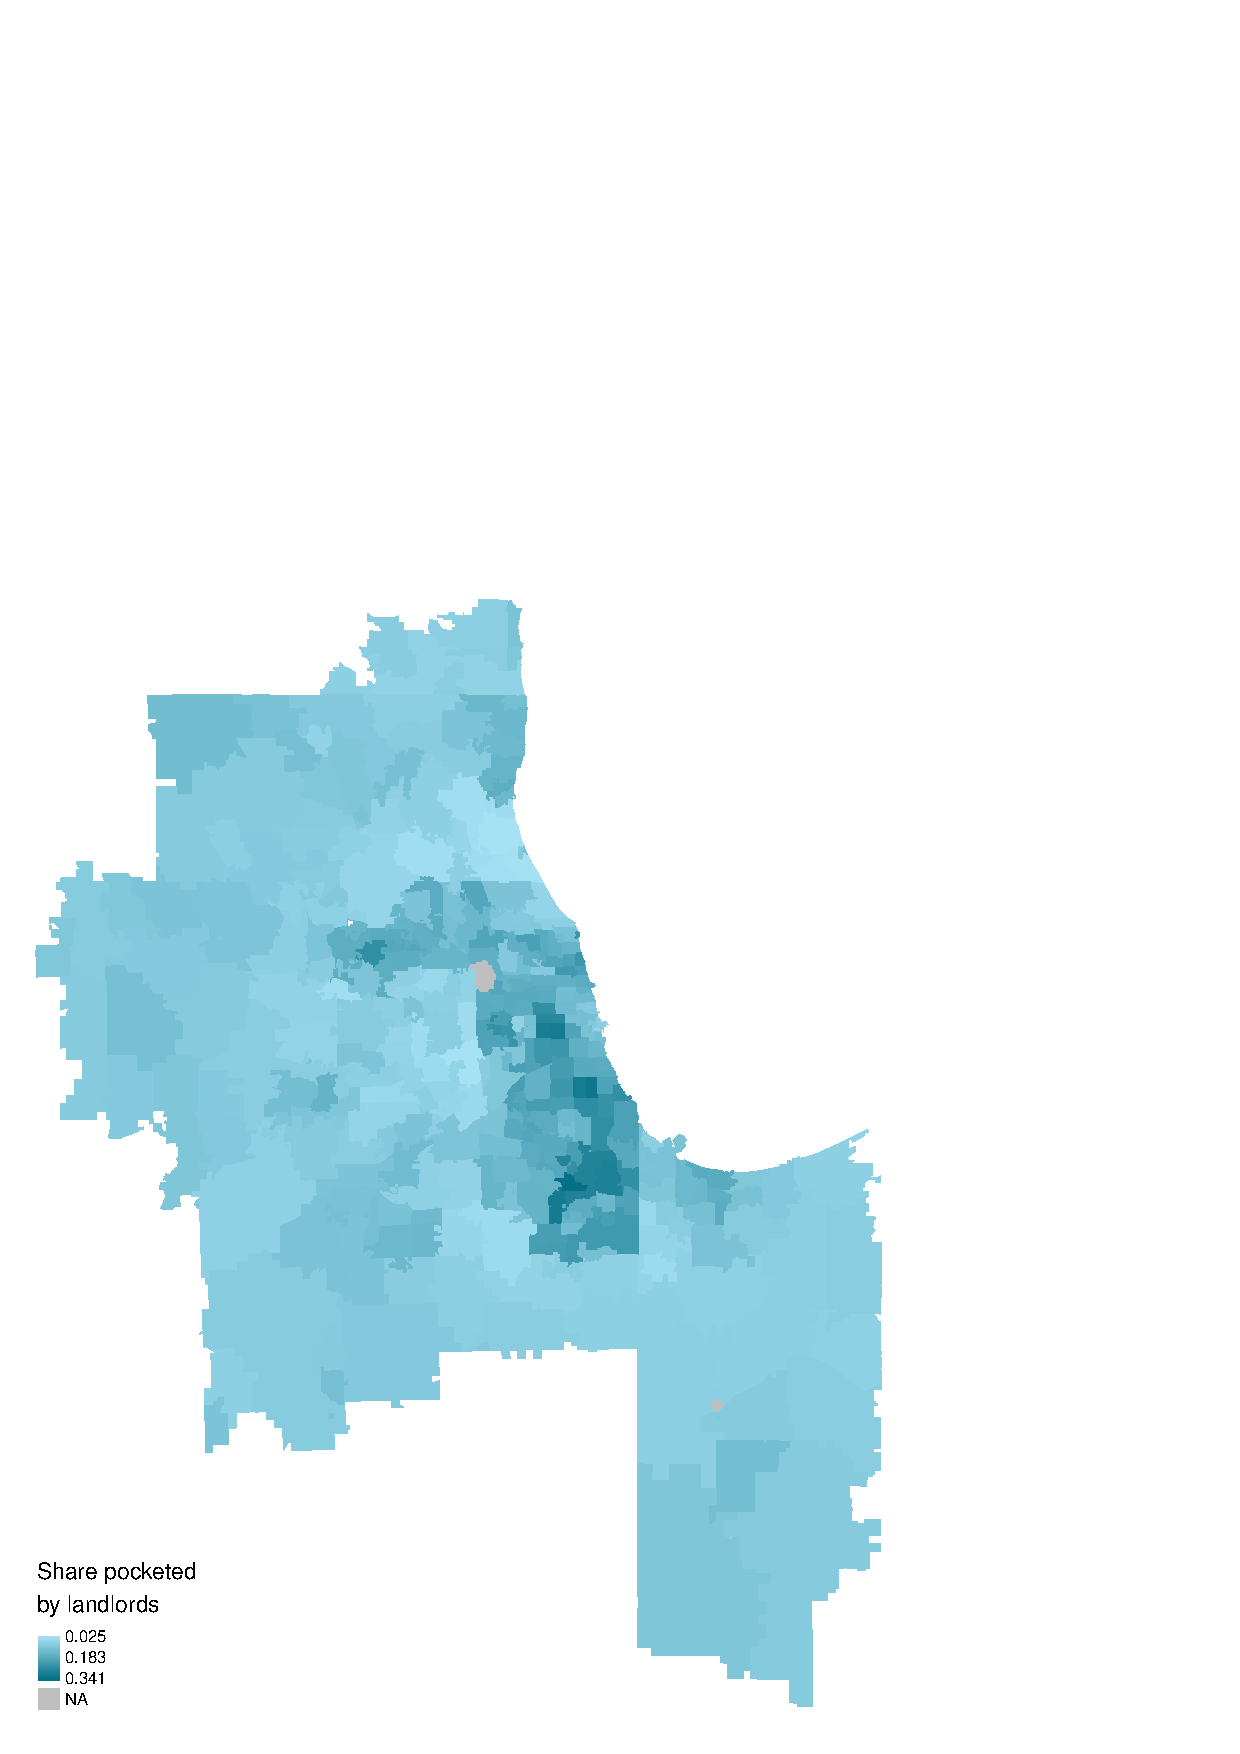
\includegraphics[width = 1\textwidth]
            {counterfactuals/output/chicago_rho_with_imputed_fed_9usd}
    \end{subfigure}%
    \begin{subfigure}{.5\textwidth}
        \caption{Increase in Chicago MW to \$14}
        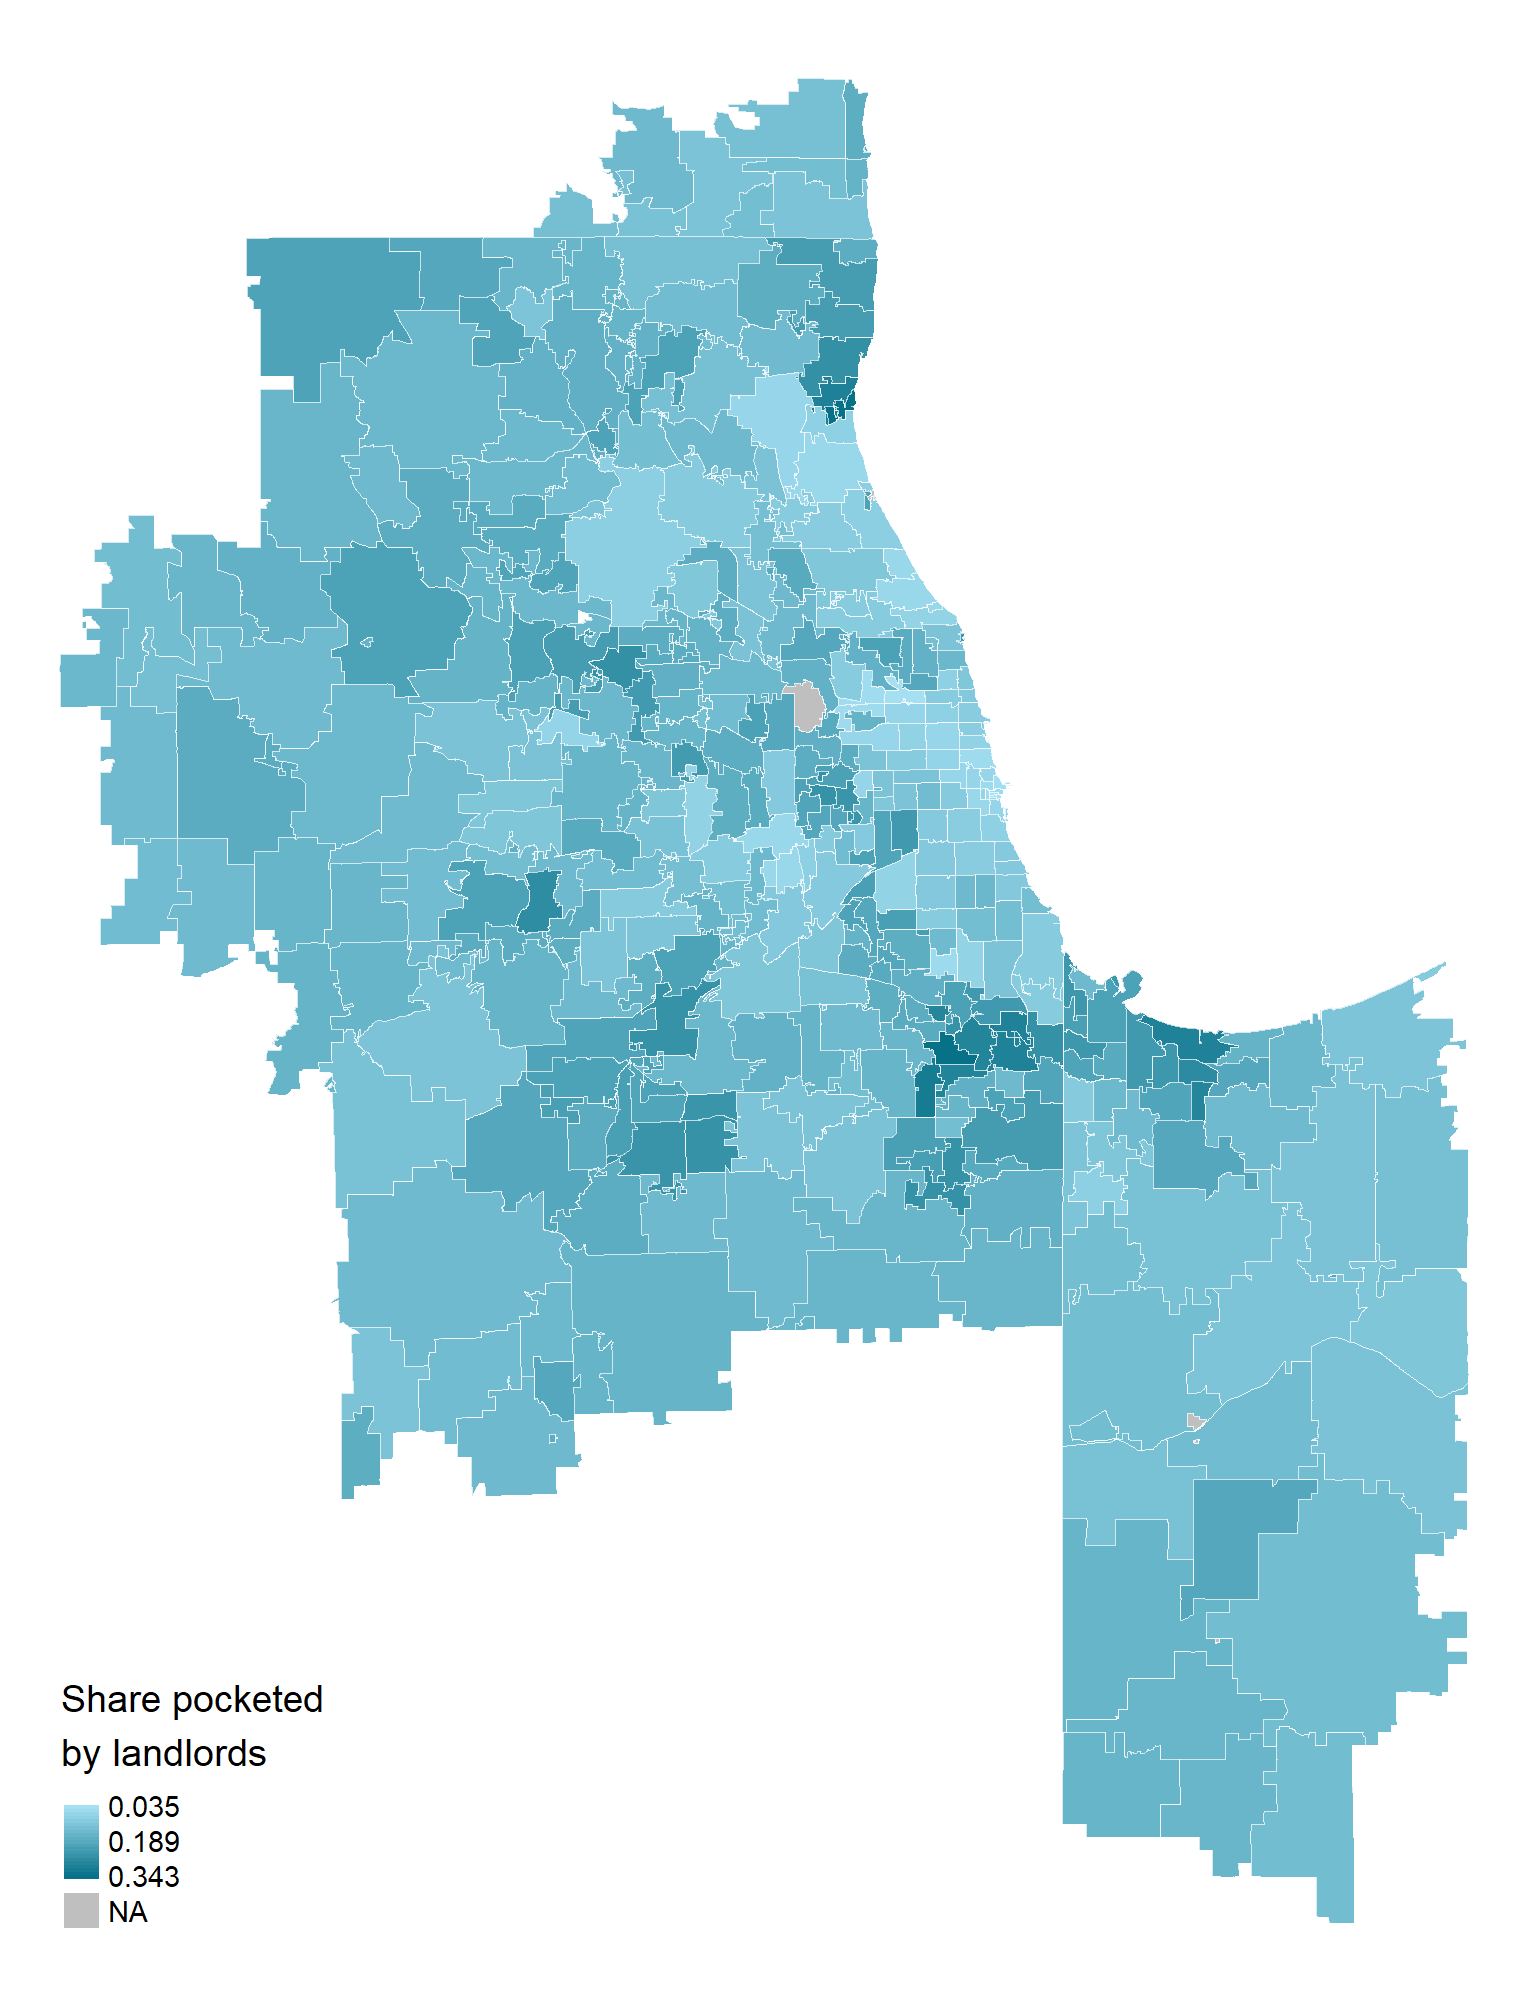
\includegraphics[width = 1\textwidth]
            {counterfactuals/output/chicago_rho_with_imputed_chi14}
    \end{subfigure}\\

    \begin{minipage}{.95\textwidth} \footnotesize
        \vspace{3mm}
        Notes: 
        Data are from the minimum wage panel described in Section 
        \ref{sec:data_mw_panel} and from LODES.
        The figures map the estimated ZIP-code specific shares of the 
        additional income generated by a MW policy that are pocketed by 
        landlords, for different counterfactual MW policies.
        Panel (a) is based on a counterfactual increase to \$9 in the 
        federal MW in January 2020, holding constant other MW policies in their 
        December 2019 levels.
        Panel (b) is based on a counterfactual increase from \$13 to \$14 in the 
        Chicago City MW, also holding constant other MW policies.
        The share pocketed is defined as the ratio between the percent increase 
        in rents and the percent increase in total wages multiplied by the share 
        of housing expenditure in the ZIP code.
        To estimate it we follow the procedure described in Section 
        \ref{sec:counterfactual}, assuming the following parameter values: 
        $\beta = \betaCf$, $\gamma = \gammaCf$, and $\varepsilon = \epsilonCf$.
    \end{minipage}
\end{figure}
